\section{Introduction}
\section{Settings}
A hand in motion can be described by two types of parameters.
\begin{itemize}
\item Pose parameters \textit{(joint angles and rigid rotation and translation of the hand)} $\theta \in \mathbb{R}^{N_{\theta}}$ change with time. 
\item Shape parameters \textit{(length and thickness of fingers phalanges, position of finger bases, shape of the palm)} $\beta \in \mathbb{R}^{N_{\beta}}$ vary between different people while staying constant for each person. 
\end{itemize}
Given a sequence of depth sensor images $\mathcal{D}_n$, the goal of our system is to get best possible estimate of shape parameters $\hat{\beta}_n$ from the input available so far.

How much information do we need to have a good guess of $\beta$? A trivial lower bound would finding $\beta$ from a single sensor image. This scenario could be conceived for palm shape and fingers thickness, since they are ``visible'' in any hand pose. However, the phalanges length cannot be estimated when the fingers are straight; moreover the locations of finger bases are hidden under the skin and can only be inferred after seeing a range of hand poses. Sensor noise and $2,5 D$ nature of the data further aggravate the problem. 
Previous authors \cite{joseph2016fits} and \cite{tkach2016sphere} suggested to find hand shape from a set of manually picked hand poses. 

\textbf{Advantages of online optimization over batch optimization}
\begin{itemize}
\item \textit{user experience:} the user does not have to track with uncalibrated model first, manually pick the poses, wait till batch optimization finishes; also there is an immediate feedback on the result quality, so no need for several ``blind'' trials.
\vspace{-1em}
\item \textit{system efficiency:} there is not need to solve a potentially very big linear system, thus hand tracking algorithm will use less computational resources; potentially it can run on a lighter hardware.
\item \textit{result quality:} this claim will be /*hopefully*/ proven experimentally. 

\begin{itemize}
\vspace{-1em}
\item By default performance of batch algorithm is an upper bound for online algorithm running on the same data. However, in practice online algorithm can use any amount of data and batch algorithm is limited by the available memory and computational power.
\item  Also, it is important that to take into account that the problem is solved with local optimization. If each frame of batch optimization is initialized far away from the true hand parameters, the solver can get stack in bad local optimum. (Shape prior should help in this case, but a good prior is difficult to learn). Online optimization, if it works properly, can have better and better initialization with every frame.
\end{itemize}
\end{itemize}

\subsection {Hand Model}

\begin{figure}[h!]
\centering
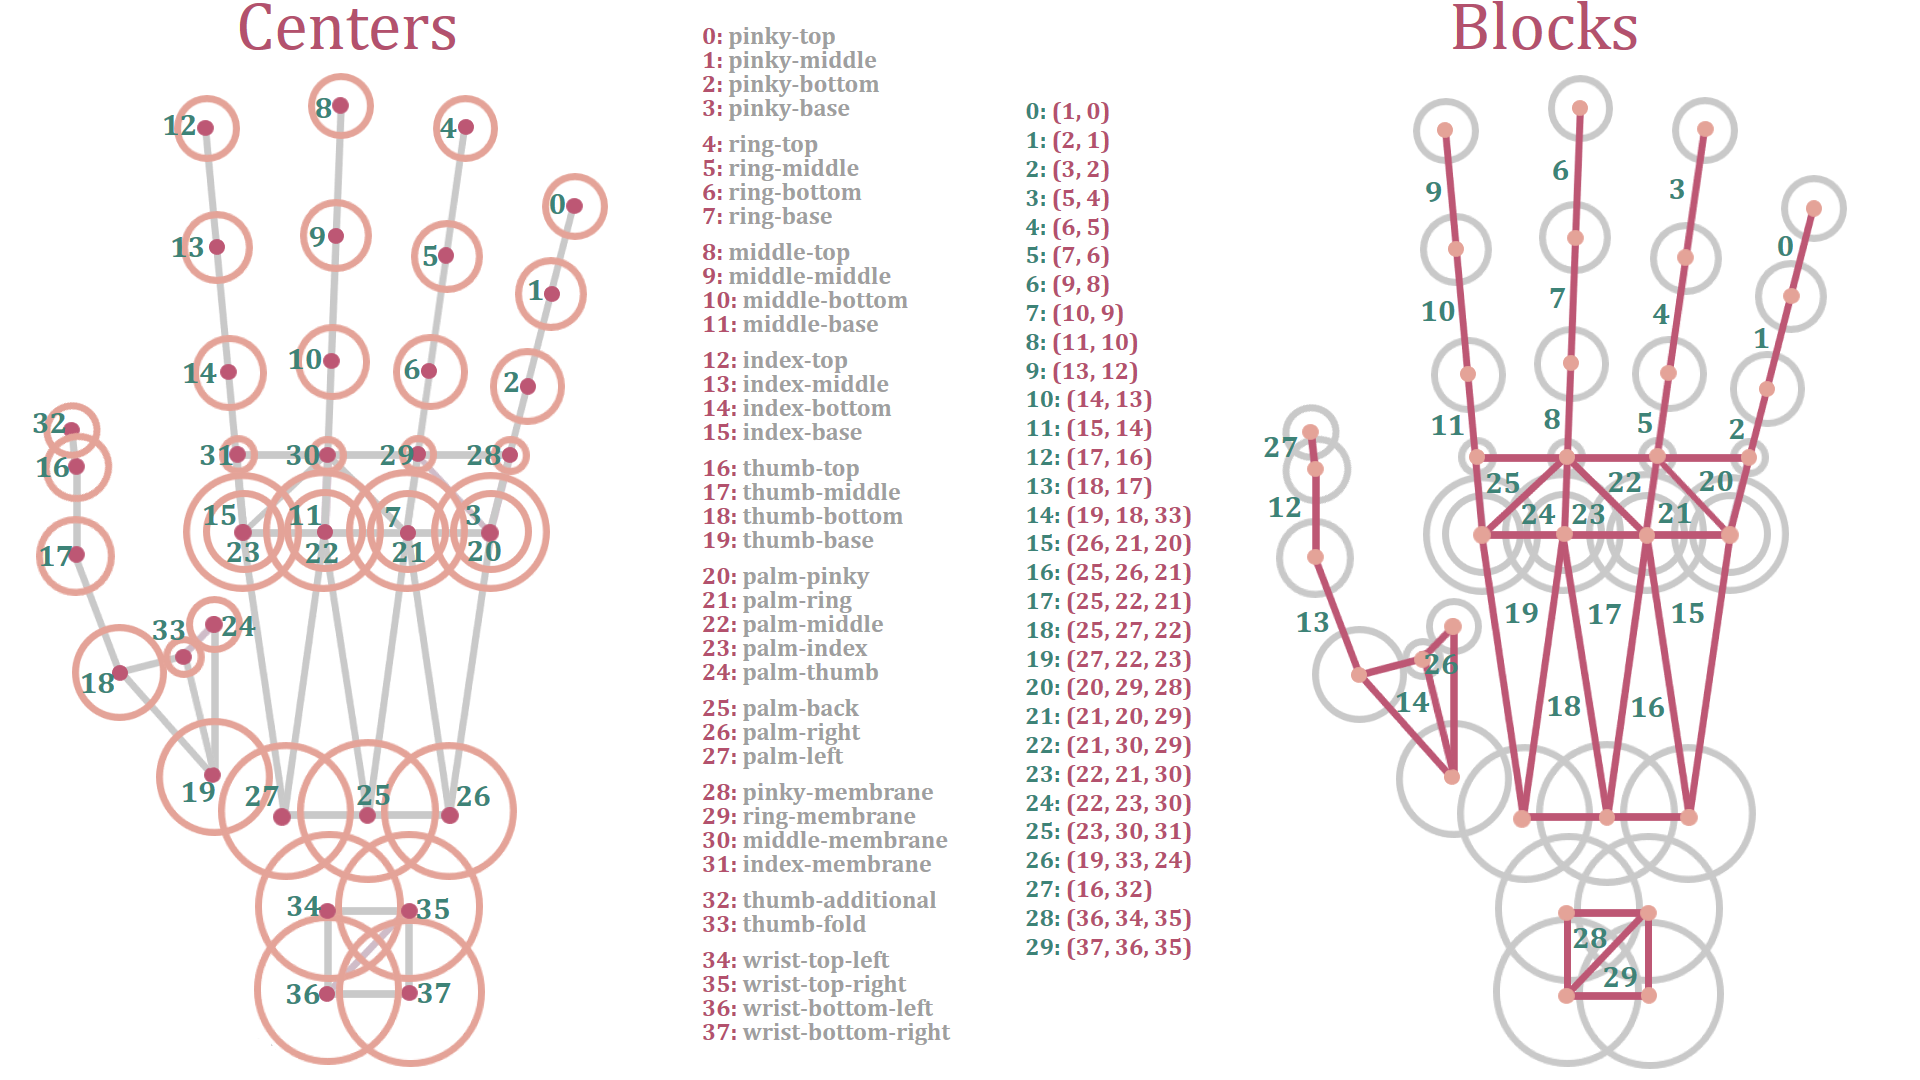
\includegraphics[width=1\linewidth]{figures/centers-blocks}
\caption{Sphere-mesh representation}
\label{fig:centers-blocks}
\end{figure}

\begin{figure}[h!]
\centering
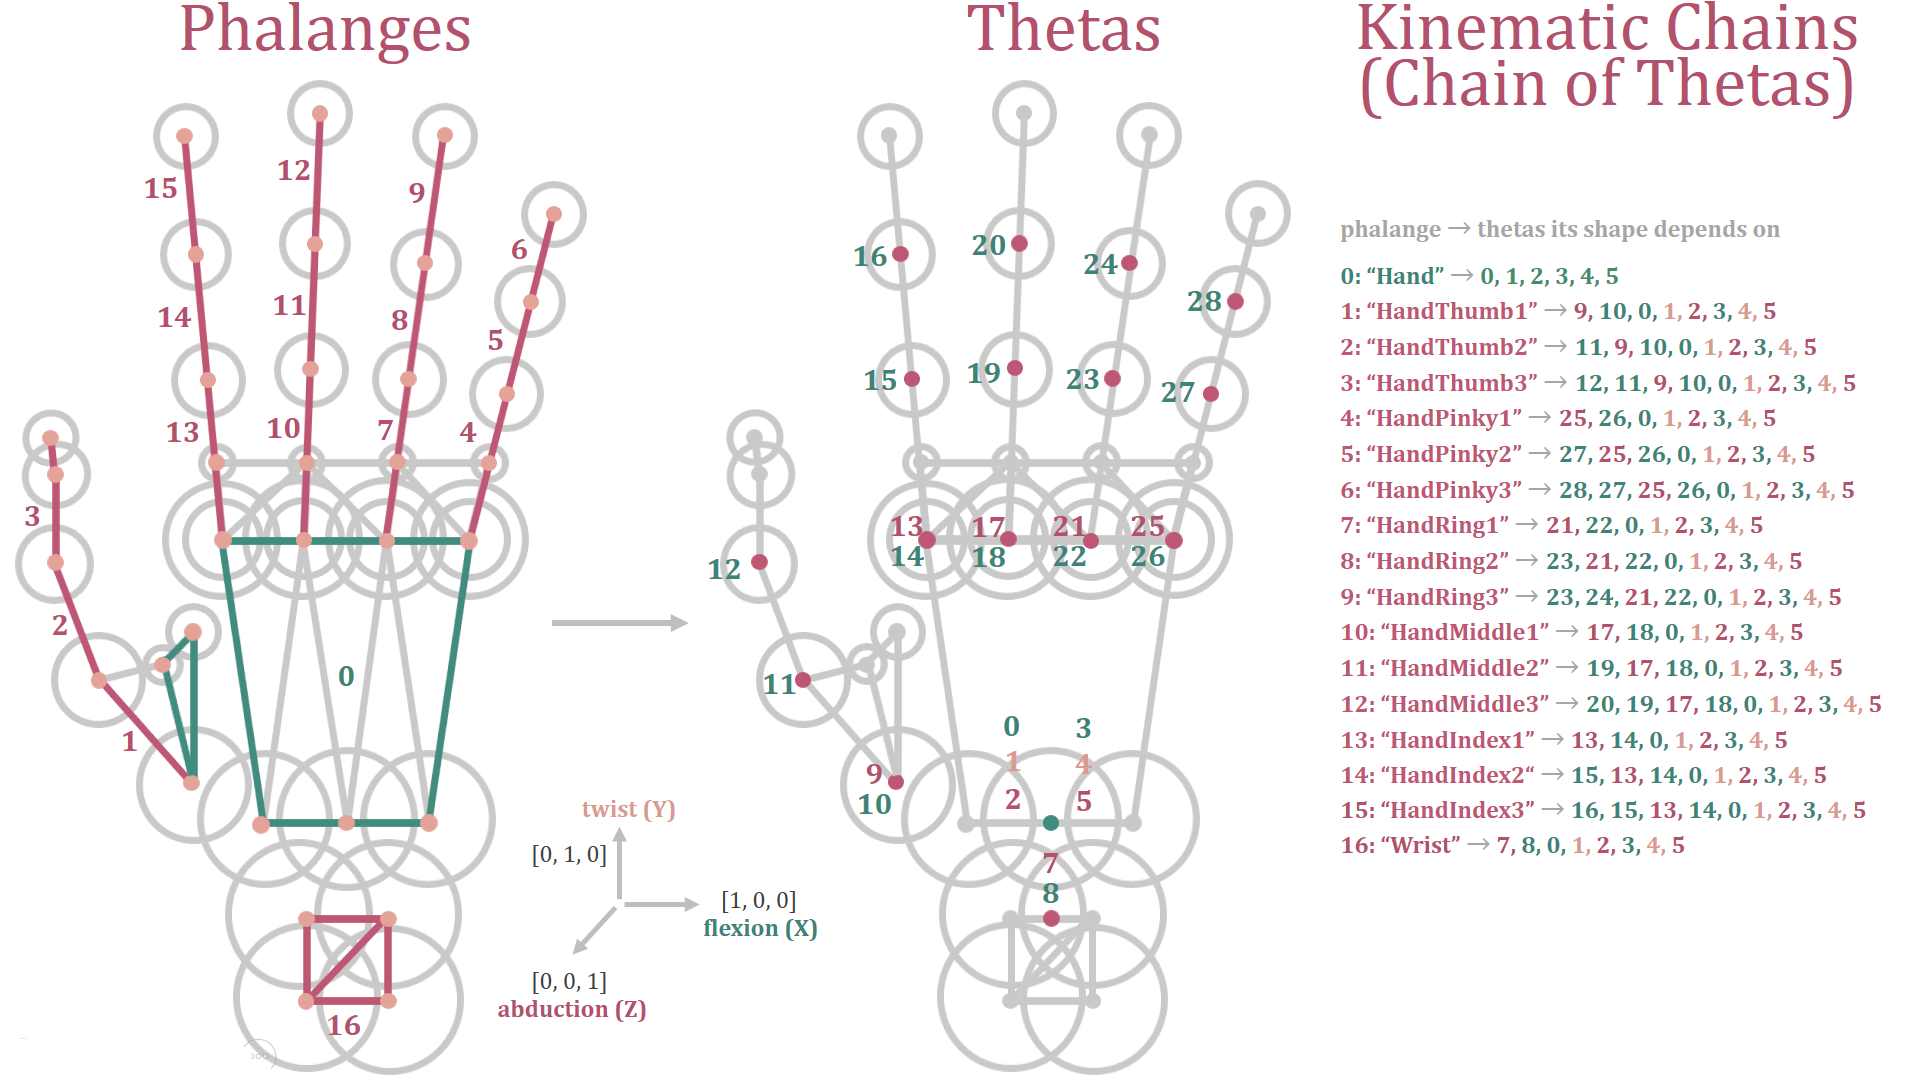
\includegraphics[width=1\linewidth]{figures/thetas}
\caption{Pose parameters $\theta$}
\label{fig:thetas}
\end{figure}

\begin{figure}[h!]
\centering
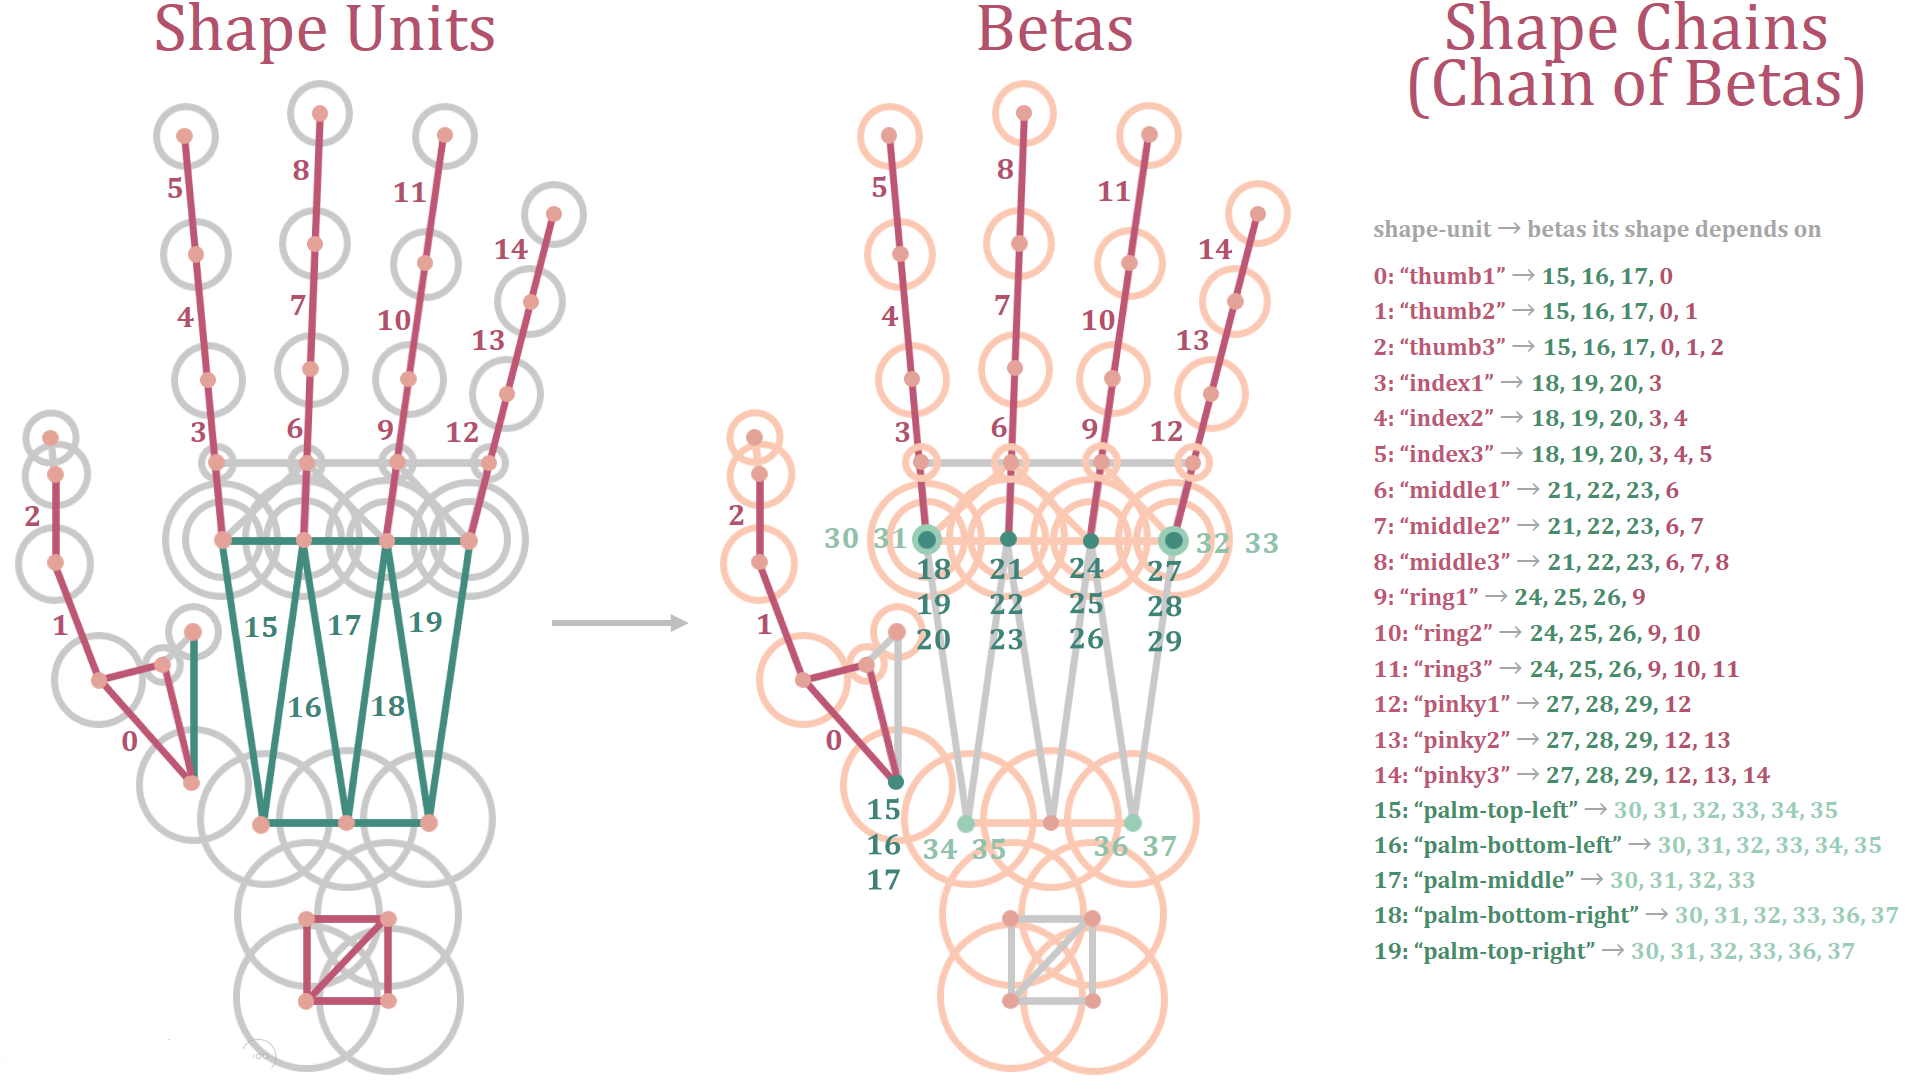
\includegraphics[width=1\linewidth]{figures/betas}
\caption{Shape parameters $\beta$}
\label{fig:betas}
\end{figure}

We use sphere-mesh hand model presented in \cite{tkach2016sphere}, which is a special case of a convolution surface. \textbf{\color{accent}{Maybe briefly recap advantages of sphere-meshes hand model representation}}. 

The skeleton $\mathcal{S} = \{\mathcal{V}, \mathcal{E}, \mathcal{F}\}$ of the sphere-mesh is a planar graph with a fixed topology. Each vertex $\mathcal{V}_i$ corresponds to a sphere with center $c_i \in \mathbb{R}^3$ and radius $r_i \in \mathbb{R}^+$. The radii at intermediate points are given by linear interpolation of the radii at the vertices.
While the skeleton topology is predefined for the class of object ``human hand'', changing centers and radii spans the pose and shape space of human hands.

Note that shape parameters $\beta$ stay constant for a given person and play a different semantic role from pose parameters $\theta$, thus it is helpful to distinguish between to two types of the parameters. Also, it is important to prohibit the degrees of freedom that are not available to the human hand. Thus we use the two representations interchangeably - sphere-meshes representation for closest point correspondences and for rendering and ``semantic'' representation for finding $\beta$ and $\theta$.
The centers $c_i$ are computed from $\beta$ and $\theta$ using forward kinematics with $\beta$ being transitional degrees of freedom and $\theta$ - rotational degrees of freedom. The ``impossible'' degrees of freedom are eliminated by only allowing only biologically plausible rotational DOFs at the joints.

\subsection {Parametrization}

A point on the model surface $m_i$ is defined by its barycentric coordinates $\{\kappa_1, \kappa_2, \kappa_3\} $ of its projection $s_i$ on the corresponding skeleton face $\mathcal{F}_j = \{c_{j1}, {c_j}_2, {c_j}_3\}$ and the offset direction $o_i \in \mathbb{R}^3$

\begin{equation}
o_i = G_j^{-1} \frac{m_i - s_i} {\| m_i - s_i \|_2^2}
\end{equation}

where $G_j$ is global transformation of the face $F_j$ given by forward kinematics.

Given the new parameters $\{ \beta', \theta' \}$, the new position of the point is
\begin{align}
\begin{split}
m_i'(\beta', \theta') = \kappa_1 c_{j1}' + \kappa_2 c_{j1}' + \kappa_3 c_{j3}' + \\
 + \;  G_j'(\kappa_1 r_{j1}' + \kappa_2 r_{j2}' + \kappa_3 r_{j3}') o_i
\end{split}
\end{align}

with $c_{j1}' = c_{j1}'(\beta', \theta')$,  $r_{j1}' = r_{j1}'(\beta', \theta')$, $G_j' =G_j'(\theta')$.